
%%%%%%%%%%%%%%%%%%%%%%%%%%%%%%%%%%%%%%%%%
% Journal Article
% LaTeX Template
% Version 1.3 (9/9/13)
%
% This template has been downloaded from:
% http://www.LaTeXTemplates.com
%
% Original author:
% Frits Wenneker (http://www.howtotex.com)
%
% License:
% CC BY-NC-SA 3.0 (http://creativecommons.org/licenses/by-nc-sa/3.0/)
%
%%%%%%%%%%%%%%%%%%%%%%%%%%%%%%%%%%%%%%%%%
%----------------------------------------------------------------------------------------
%       PACKAGES AND OTHER DOCUMENT CONFIGURATIONS
%----------------------------------------------------------------------------------------
\documentclass[paper=a4, fontsize=12pt]{article}
\usepackage[english]{babel} % English language/hyphenation
\usepackage[protrusion=true,expansion=true]{microtype} 
%\usepackage[protrusion=true]{microtype} 
\usepackage{amsmath,amsfonts,amsthm} % Math packages
\usepackage{mathtools}
%\usepackage[utf8]{inputenc}
\usepackage{color}
\usepackage{blindtext}
\usepackage{graphicx} 
\usepackage{subcaption}
%\usepackage[sc]{mathpazo} % Use the Palatino font
\usepackage{epstopdf}
%\usepackage[cm]{sfmath}
%\usepackage{cmbright}
%\usepackage[math]{kurier}
%\usepackage{fourier}
%\usepackage{pxfonts}
%\usepackage[math]{iwona}
\usepackage[charter]{mathdesign}
\usepackage[T1]{fontenc} % Use 8-bit encoding that has 256 glyphs
\linespread{1.05} % Line spacing - Palatino needs more space between lines
%\usepackage{microtype} % Slightly tweak font spacing for aesthetics
%\usepackage{chemformula}
\usepackage[hidelinks]{hyperref}
\usepackage[hmarginratio=1:1,top=32mm,columnsep=20pt]{geometry} % Document margins
\usepackage{multicol} % Used for the two-column layout of the document
%\usepackage[hang, small,labelfont=bf,up,textfont=it,up]{caption} % Custom captions under/above floats in tables or figures
\usepackage{booktabs} % Horizontal rules in tables
\usepackage{tabularx}
\usepackage{float} % Required for tables and figures in the multi-column environment - they need to be placed in specific locations with the [H] (e.g. \begin{table}[H])
\usepackage{hyperref} % For hyperlinks in the PDF
\usepackage{lettrine} % The lettrine is the first enlarged letter at the beginning of the text
\usepackage{paralist} % Used for the compactitem environment which makes bullet points with less space between them
\usepackage{abstract} % Allows abstract customization
\renewcommand{\abstractnamefont}{\normalfont\bfseries} % Set the "Abstract" text to bold
\renewcommand{\abstracttextfont}{\normalfont\small\itshape} % Set the abstract itself to small italic text
\usepackage{titlesec} % Allows customization of titles
\usepackage{enumitem}

\renewcommand\thesection{\Roman{section}} % Roman numerals for the sections
\renewcommand\thesubsection{\Roman{subsection}} % Roman numerals for subsections

\titleformat{\section}[block]{\large\bfseries}{\thesection.}{1em}{} % Change the look of the section titles
\titleformat{\subsection}[block]{\large}{\thesubsection.}{1em}{} % Change the look of the section titles
\newcommand{\horrule}[1]{\rule{\linewidth}{#1}} % Create horizontal rule command with 1 argument of height
\usepackage{fancyhdr} % Headers and footers
\pagestyle{fancy} % All pages have headers and footers
\fancyhead{} % Blank out the default header
\fancyfoot{} % Blank out the default footer
\renewcommand{\headrulewidth}{0pt} % no top rule

\fancyhead[C]{} % Custom header text

\fancyfoot[RO,LE]{\thepage} % Custom footer text
%----------------------------------------------------------------------------------------
%       TITLE SECTION
%----------------------------------------------------------------------------------------
\title{\vspace{-15mm}\huge SimStrat \\ 1D k-epsilon lake model \\[0.5cm] \textbf{Developer Manual}} % Article title
\author{
\large
{\textsc{}}\\[2mm]
}
\date{}

%----------------------------------------------------------------------------------------
\begin{document}

\begin{titlepage}
	\maketitle % Insert title
	\thispagestyle{empty}
	\tableofcontents
	\vspace{5cm}
	\begin{figure}[h]
		
\includegraphics[width=0.3\textwidth]{ealogo05-150.eps}
	\end{figure}

	\noindent\fontfamily{phv}\selectfont Swiss Federal Institut of Aquatic Science and Technology, December 2016
\end{titlepage}
\thispagestyle{fancy} % All pages have headers and footers

\section{Introduction}
This developer manual is ...

\section{Requirements}

make

Cmake

GNU-Fortran compiler

Alternatively Intel Fortran Compiler

\section{Download and install SimStrat}

\newpage
\section{Code Structure}
The code structure of simstrat has been updated to an object-oriented model. In this chapter, the main architecture is documented and a short description of each used class is given. Additionally, the important classes for solving model variables and for updating the grid are explained in more detail.

\subsection{Overview}
The following class diagram gives an overview of the coupling of the different classes.
\begin{figure}[h]
		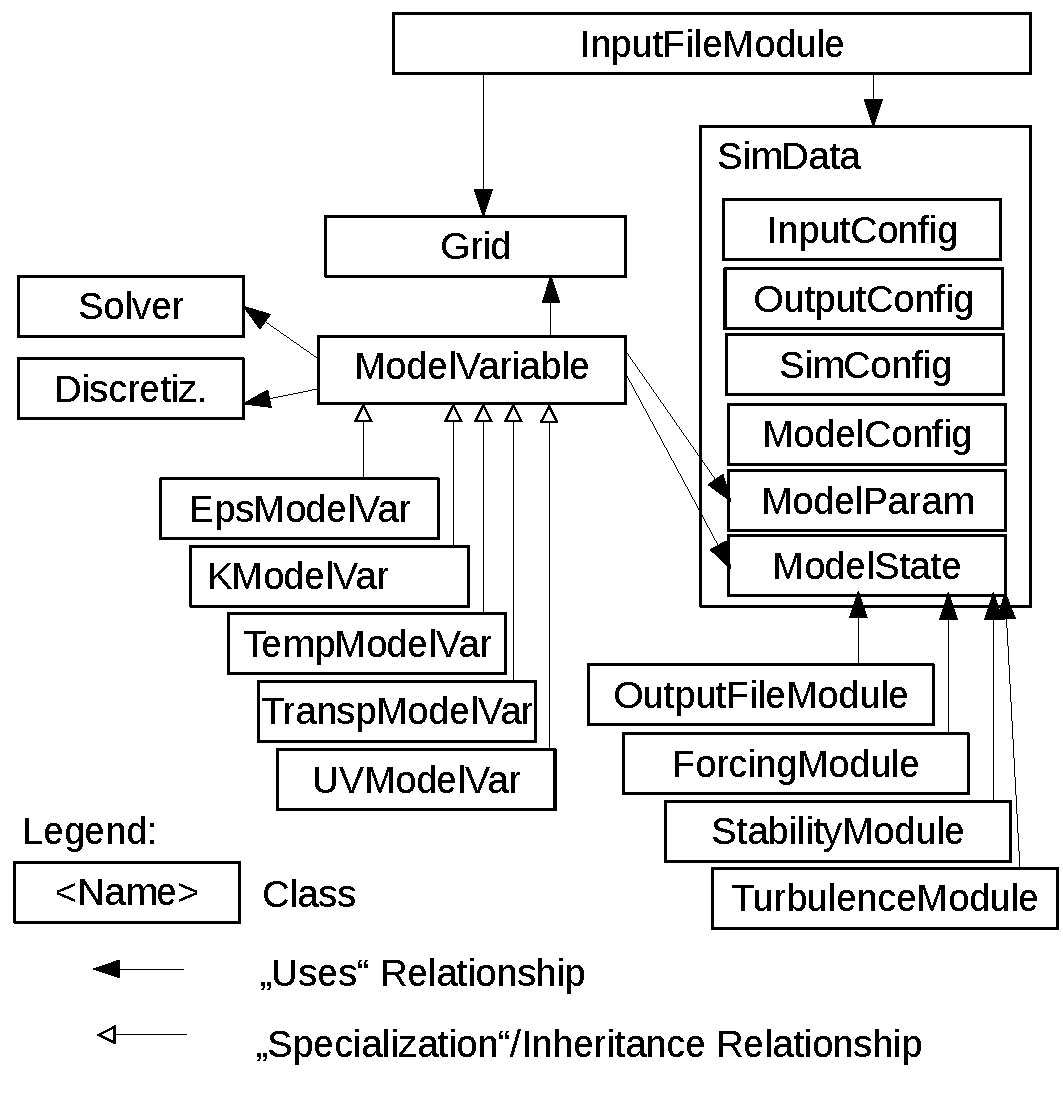
\includegraphics[width=0.75\textwidth]{classdiagram.pdf}
		\caption{Class diagram of Simstrat2.}
\end{figure}
The main points of the architecture are:
\begin{itemize}
	\item All simulation data is kept inside the SimData class and its various subclasses. Additionally, a grid class containing all information and methods (update/interpolate etc) concerning the grid is kept. This information is all read and set up by the InputFileModule.
	
	\item All variables that need to be solved to update $(K,\epsilon,T,S,U,V)$ have a corresponding module that contains the logic to calculate the terms needed for constructing a linear system of equations. All these modules are inherited from an abstract base class "ModelVariable" that provides the logic to combine solver, grid, discretization and variable data. Each inherited subclass only overwrites the needed methods (usually calc\_terms).
	
	\item Most other parts of the software, such as output data storage, forcing or (stability-)parameter updates are structured into single classes that have access to the model state and/or grid.
\end{itemize}

Once the simulation has been set up, only the update methods of each module are called during each iteration:
\begin{enumerate}
	\item Update current simulation date
	\item Read \& update forcing data (ForcingModule update)
	\item Read \& update in/outflows
	\item Update stability data $N^{2},cmue$ (StabilityModule update)
	\item Update $U$ and $V$ (UVModelVar update)
	\item Update $T$ (TempModelVar update)
	\item Update $S$ (TranspModelVar update)
	\item Update turbulence data $P,P_{seiche},\nu_{m},\nu_{h}$ (TurbulenceModule update)
	\item Update $k$ (KModelVar update)
	\item Update $eps$ (EpsModelVar update)
	\item Call logger to log current state
\end{enumerate}

\newpage
\subsection{Classes}

The following classes/modules/interfaces are of importance:

\begin{description}[style=nextline]
	\vspace{1em}
	\hrule
	\item[Interfaces] \noindent Interfaces that may have multiple implementations to facilitate different variants
	
\begin{description}[style=multiline, leftmargin=17em]
		\item[LinSysSolver] Interface for a linear system solver, that solves for $x$ in $Ax=b$, where $A$ is tridiagonal.
		
		\item[SimstratOutputLogger] Interface that describes an output module which writes simulation data for further processing (e.g. CSV files or Matlab files etc)
		
		\item[ModelVariable] Interface that defines a generic object that manipulates a model variable (e.g. Transport equation, or update of windshear etc). Contains an abstract update method that performs the update process depending on the actual parametrization:
			\begin{enumerate}
				\item "Calculate terms": This calls the subroutine to calculate the source terms and boundary conditions. This method is abstract and has to be overwritten by the effective implementation.
				\item Create linear system of equations: Uses the associated discretization method to create a tridiagonal matrix A and the right hand side.
				\item Solve: Uses the associated solver to solve the before created linear system
				\item "Post Solve": Execute a method to manipulate the variable after solving - default implementation is just an empty method but can be overwritten as needed.
			
			\end{enumerate}


	\item[Discretization] Defines the interface for discretization classes that, based on input quantities such as fluxes, current states and timestep, construct a linear system of equation.
\end{description}
 \hrule
 
 	\item[DTOs] \noindent Data transfer objects that mainly store data, but do not manipulate them (except e.g. converting data)
 \begin{description}[style=multiline, leftmargin=17em]
		\item[InputConfig] Holds file system path of all input files
		
		\item[OutputConfig] Holds file system path for all output files and additional information such as logging frequency and similar
		
		\item[SimConfig] Stores fixed simulation configuration, such as start/end date and timestep. 

		\item[ModelConfig] Stores fixed model configuration, such as turbulence model selection or forcing mode.
		
		\item[ModelParam] Stores fixed model parameters, such as Latitude or $\rho_{air}$
		
		\item[ModelState] All model variables (i.e. everything that changes during an iteration)
\end{description}

 \hrule
\item[Special classes] \noindent Utility and helper classes  
 \begin{description}[style=multiline, leftmargin=17em]
		\item[Inputfile] Module that reads all the input files and populates the aforementioned data transfer objects. Sets up the simulation.
		
		\item[Grid] Contains all information and routines concerning the grid. Both grids (centered on face / centered on volume) are stored and updated in this class. Additionally, methods such as interpolating from/to a grid and updating area factors belong to the grid.
		
		\item[Forcing] Parses forcing files and updates the current ModelState according to the date.

		\item[Stability] Manipulates the NN and cmue1/2 variables of the ModelState
\end{description}

		\item[Absorption] Reads absorption input file and modifies corresponding variables of the Modelstate
		
		\item[Lateral] Reads input files for in/outflows (Qinp, Qout, Tin, Sin) and integrates/interpolates values in order to modify $Q_{inp}$/$Q_{vert}$
		
		\item[Advection] Based on already read in/outflows ($Q_{inp}$/$Q_{vert}$), calculates the advection terms

 \hrule
\item[Model state variable classes] \noindent Classes that are inherited from ModelVariable
 \begin{description}[style=multiline, leftmargin=17em]
		\item[TranspModelVar] Simplest inherited class from ModelVariable.  Contains additional method to assign an external source term. Overwrites calc\_terms and sets source terms to the afore mentioned source terms. This class can be used for all quantities that need to be transported/distributed without special boundary conditions/equations. Examples include salinity $S$ and additional biogeochemical quantities.
		
		\item[TempModelVar] Used for $T$ variable. In the calc\_terms function, radiance into each layer is calculated and added as a source term. Additionally, boundary fluxes according to geothermal/boundary heat fluxes are added.
		
		\item[UVModelVar] Used for $U$/$V$ variable. Same class can be instantiated twice and assigned to $U$ respectively $V$, as the code is the same. Additional to the variable, a shear stress variable has to be defined using the assign\_shear\_stress method.
		
		\item[KModelVar] Used for $K$ variable. Contains calculation for sources/boundary conditions needed to calculate $K$. Contains post\_solve function to adjust first/last element of $K$ after solve

		\item[EpsModelVar] Used for $\epsilon$ variable. Similar to KModelVar.
\end{description}
\end{description}



\subsection{Implementation of an equation}
In this chapter, the detailed approach how a state variable is solved is explained (mostly for code documentation purposes - for more information about the math/discretization used, see next chapters).



\subsection{Grid}
All methods and variables concerning the grid structure are now combined into a grid class.
The grid class takes care of 
\begin{itemize}
	\item Updating area factors
	\item Storing the two grids (volume and face) including heights, areas etc
	\item Growing/merging grid boxes if needed
	\item updating upper bounds and sizes
	\item Interpolate from and to the grid (e.g. interpolate a value with a different z-axis onto the volume grid)
\end{itemize}

Note that there 2 grids - one that stores the depth of each face, and one that stores the depth of each volume center.
Consequently, they are named \texttt{z\_face} respectively \texttt{z\_volume}. Both are 1-indexed and \texttt{z\_face} is always one element longer than \texttt{z\_volume}. The current upper bounds for both grids can be queried using the \texttt{ubnd\_fce} and \texttt{ubnd\_vol} variable in the grid class. 

These upper bounds are automatically updated using the \texttt{update\_nz} method, e.g. when shrinking/growing the grid.


\subsection{Output logger} 
The interface \texttt{SimstratOutputLogger} in file \texttt{strat\_outputfile.f03} defines a generic logger. Currently, \texttt{SimpleLogger} is implemented.

Configuration of the logger is done using the \texttt{output\_cfg} variable in the \texttt{simdata} structure. It consists of an array of pointers and descriptions, so that the logger knows which variables has to be saved to which file. 

Example:
\begin{verbatim}
self%simdata%output_cfg%output_vars(1)%name = "V"
self%simdata%output_cfg%output_vars(1)%values => self%simdata%model%V
self%simdata%output_cfg%output_vars(1)%center_grid = .true.
\end{verbatim}

This tells the logger to output variable \texttt{self\%simdata\%model\%V} as variable with the name "V" on the volume grid, whenever the log function is called.

\subsection{Proposed Coupling to AED2}

\subsubsection{Input files}

\subsubsection{Transport Modelvariable}

\subsubsection{Update}

\subsubsection{Output files}

\subsection{Further work on the implementation}
The current state (Spring 17) of the code should give a solid foundation for further development. It is by no means ideal - it is more a high-level restructuring than a in-depth refactoring of each part/method. Thus, there are still a lot of things to improve. This chapter should give some ideas on what could be further improved.

\begin{itemize}
	\item Clean code and readability: Lot of ambigious named variables and hard to debug if/else constructs with code duplication. Methods (e.g. the lateral method) are sometimes very long and could probably be restructured into a combination of well named, short and easy to test methods. 
	
	\item File reading of input files: Very hard to debug, very unclear and old-style goto- failure modes. For long term development, this should be refactored out into a generic time-series class that can read the desired file format and returns it as a 2d array or so. This class could then be re-used in all modules that have to read input files (such as Qin, Qout, Tin etc).
	
	\item List of methods that badly need refactoring:
	\begin{itemize}
		\item \texttt{forcing\_update}: Much too long. Should be multiple, well named subfunctions instead of long if/else structure
		
			\item \texttt{everything in lateral}: same as above
	\end{itemize}

\end{itemize}


\section{Discretization Scheme and Numerical Approach}
\subsection{System of Governing Equations}
The governing equations are described in Goudsmit et al. 2000
\begin{align}
	\frac{\partial T}{\partial t} &= \frac{1}{A}\frac{\partial}{\partial z}\left(A(\nu'_t + \nu')\frac{\partial T}{\partial z}\right)+\frac{1}{\rho_0 c_p}\frac{\partial H_{sol}}{\partial z}+\frac{dA}{dz}\frac{H_{geo}}{A\rho_0 c_p}\\
	\begin{split}
		\frac{\partial u}{\partial t} &= \frac{1}{A}\frac{\partial}{\partial z}\left(A(\nu_t + \nu)\frac{\partial u}{\partial z}\right) + fv\\
		\frac{\partial v}{\partial t} &= \frac{1}{A}\frac{\partial}{\partial z}\left(A(\nu_t + \nu)\frac{\partial v}{\partial z}\right) - fu
	\end{split}\\
	\frac{\partial k}{\partial t} &= \frac{1}{A}\frac{\partial}{\partial z}\left(A\nu_k\frac{\partial k}{\partial z}\right) + P + P_{seiche} + B - \epsilon\\
	\frac{\partial \epsilon}{\partial t} &= \frac{1}{A}\frac{\partial}{\partial z}\left(A\nu_{\epsilon}\frac{\partial \epsilon}{\partial z}\right) + \frac{k}{\epsilon}\left(c_{\epsilon 1}\left(P+P_{seiche}\right)+c_{\epsilon 3}B-c_{\epsilon 2}\epsilon\right)
\end{align}
Note that these equations do not include advection caused by in- and outflow caused by rivers and/or groundwater sources. In Simstrat, advection is decoupled from diffusion and source/sink treatment and computed separately.

\subsection{Numerical Concept}
In the above system of partial differential equations the temporal change of a quantity formally consists of a diffusive component $D$ and a source/sink component $S$:
\begin{equation}
	\frac{\partial\phi}{\partial t} = D(t, \phi) + S(t)
\end{equation}

\noindent For the numerical integration an implicit Euler method is applied:
\begin{equation}
	\frac{\phi^{n+1}-\phi^n}{dt} = D(t^{n+1}, \phi^{n+1}) + S(t^{n}) 
\end{equation}

\noindent The resulting system of discretized equations can be written as a system of linear equations of the form:
\begin{equation}
	R\phi^{n+1}=\phi^n+dt\cdot S^{n}
\end{equation}
where $\phi$ represents any of the above quantities ($T$, $u$, $v$, $k$, $\epsilon$), and $R$ is a tridiagonal matrix of the form:
\begin{equation}
	R=\begin{bmatrix}
	bu		&	au		&	0		&	\hdots	&	0  \\
	cu		&	bu		&	au		&	 		&	\vdots \\
	0		&	\ddots	&	\ddots	&	\ddots	&	0 \\
	\vdots	&			&	\ddots	&	\ddots	&	au \\
	0		&	\hdots	&	0		&	cu		&	bu
	\end{bmatrix}
\end{equation}
where $bu=(1-au-cu)$. This system of linear equations can be solved very efficiently by the tridiagonal matrix algorithm.

\subsection{Discretization Scheme: Finite Volume Approach on a Staggered Grid}
The discretization follows a finite volume approach. The water column is divided into $n_{vol}$ volumes with height $h_z$, an area $A_{z+1}$ at the top of the volume and $A_{z-1}$ at the bottom (the so-called faces). The volume centers have indices from 1 to $n_{vol}$ (bottom to surface). The faces have indices from 1 to $n_{face}$ which is equal to $n_{vol}+1$. The mean flow quantities ($T$, $u$, $v$) are placed at the center of the volumes. Turbulent quantities ($k$, $\epsilon$) are assigned to the volume faces (the interface between two volumes). Within a volume, the diffusion coefficients are assumed to be equal to the mean value of the diffusion coefficients at the upper and lower face.

\begin{figure}[h!]
	\centering
	\def\svgwidth{\textwidth}
	\input{SimstratDiscretizationScheme_edited.pdf_tex}
	\caption{Discretization Scheme}
\end{figure}

The temporal change of mean flow quantities within each volume results from the diffusive fluxes through the two interfaces and sources/sinks within the volume:
\begin{equation}
	\left.\frac{\partial\phi}{\partial t}\right|_{z} = \frac{A_{z}F_{z}-A_{z+1}F_{z+1}}{V_z}+S_z
\end{equation}
where $V_z=h_z\left(A_z+A_{z+1}\right)/2$.

The flux through the upper and lower interface are:
\begin{align}
	F_{z+1,face} &= -\nu\left.\frac{\partial \phi}{\partial z}\right|_{z+1}^{face} = -\nu_{z+1}\frac{\phi_{z+1}-\phi_{z}}{(h_{z+1}+h_{z})/2} \\
	F_{z,face} &= -\nu\left.\frac{\partial \phi}{\partial z}\right|_{z}^{face} = -\nu_z\frac{\phi_{z}-\phi_{z-1}}{(h_{z}+h_{z-1})/2}
\end{align}

\noindent The resulting discretization for mean flow quantities is then:
\begin{equation}
	\frac{\phi^{n+1}_z-\phi^n_z}{dt} = \frac{1}{h_z\left(A_z+A_{z+1}\right)/2}
	\left(A_{z+1}\nu^{n}_{z+1}\frac{\phi^{n+1}_{z+1}-\phi^{n+1}_{z}}{(h_{z+1}+h_{z})/2}-A_{z}\nu^{n}_z\frac{\phi^{n+1}_{z}-\phi^{n+1}_{z-1}}{(h_{z}+h_{z-1})/2}
	\right)+S^n_z 
\end{equation}

\noindent This can be rearranged to:
\begin{align}
	&dt\cdot AreaFactor_1\cdot\nu^{n+1}_z\phi^{n+1}_{z-1}\nonumber\\
	&+(1-dt\cdot AreaFactor_1\nu^{n}_z-dt\cdot form_2\nu^{n}_{z+1})\phi^{n+1}_z\nonumber\\
	&+ dt\cdot AreaFactor_2\cdot\nu^{n+1}_{z+1}\phi^{n+1}_{z+1} = \phi^{n}_{z}+dt\cdot S^n_z\\
	&AreaFactor_1 = \frac{-4A_{z}}{\left(A_z+A_{z+1}\right)\left(h_{z}+h_{z-1}\right)}\\
	&AreaFactor_2 = \frac{-4A_{z+1}}{\left(A_z+A_{z+1}\right)\left(h_{z+1}+h_{z}\right)}
\end{align}

The temporal change of turbulent quantities mainly follows the same concept except that the control volumes are shifted so that the turbulent quantities are at the center of the control volumes and the mean flow quantities are located at the volume faces. The balance for the turbulent quantities is therefore:
\begin{equation}
	\left.\frac{\partial\phi}{\partial t}\right|_{z} =
	\frac{\left(A_z+A_{z-1}\right)/2\cdot F_{z-1}-\left(A_{z+1}+A_z\right)/2\cdot F_{z}}{V_z}+S_z
\end{equation}
where $V_z=A_z\left(h_{z-1}+h_{z}\right)/2$.

To calculate the flux through the upper and lower interface the turbulent kinetic energy and the dissipation at these interfaces are approximated by averaging the TKE and dissipation at the volume centres:
\begin{align}
	\nu_{z,face}&=\left(\nu_{z,center}+\nu_{z-1,center}\right)/2 \\
\end{align}

\noindent The flux through the upper and lower interface are:
\begin{align}
F_{z,center} &= -\nu\left.\frac{\partial \phi}{\partial z}\right|_{z}^{center} = -\nu_{z}\frac{\phi_{z+1}-\phi_{z}}{h_{z}} \\
F_{z-1,center} &= -\nu\left.\frac{\partial \phi}{\partial z}\right|_{z-1}^{center} = -\nu_{z-1}\frac{\phi_{z}-\phi_{z-1}}{h_{z-1}}
\end{align}

\noindent The resulting discretization for turbulent quantities is then:
\begin{align}
&\frac{\phi^{n+1}_z-\phi^n_z}{dt} = \nonumber\\
&\frac{1}{A_z\left(h_z+h_{z+1}\right)/2}
\left(\frac{A_{z+1}+A_z}{2}\nu^{n}_{z}\frac{\phi^{n+1}_{z+1}-\phi^{n+1}_{z}}{h_{z}}
-\frac{A_{z}+A_{z-1}}{2}\nu^{n}_{z-1}\frac{\phi^{n+1}_{z}-\phi^{n+1}_{z-1}}{h_{z-1}}
\right)+S^n_z 
\end{align}

\noindent This can be rearranged to:
\begin{align}
  &\left(dt\cdot AreaFactor_{k1}\cdot\nu^{n+1}_{z-1}\right)\phi^{n+1}_{z-1}\nonumber\\
  +&\left(1-dt\cdot AreaFactor_{k1}\nu^{n}_{z-1}-dt\cdot AreaFactor_{k2}\nu^{n}_{z}\right)\phi^{n+1}_z\nonumber\\
  +&\left(dt\cdot AreaFactor_{k2}\cdot\nu^{n+1}_{z}\right)\phi^{n+1}_{z+1}\nonumber\\ 
  =& \phi^{n}_{z}+dt\cdot S^n_z\\
&AreaFactor_{k1} = \frac{A_{z}+A_{z-1}}{A_z\left(h_z+h_{z-1}\right)h_{z-1}}\\
&AreaFactor_{k2} = \frac{A_{z+1}+A_z}{A_z\left(h_z+h_{z-1}\right)h_{z}}
\end{align}


\subsection{Boundary Conditions at the Sediment and Lake Surface}

The basic discretization assumes a no-flux boundary at the sediment and lake surface. Concentration dependent fluxes at these interfaces are implemented as an additional component of the main diagonal.

%----------------------------------------------------------------------------------------
%\end{multicols}
\end{document}
